\chapter{Detection using network traffic analysis}
\label{chap:netanalysis}
In this chapter, we will discuss about malware detection using Network traffic analysis. This chapter contains 2 sections. Section~\ref{sec:netanalysisstrategy} describes the outline of our strategy, and in section~\ref{sec:netanalysismain}, we describe the procedure in details.
\section{Strategy of Malware Detection}
\label{sec:netanalysisstrategy}
At first, we created log of URLs that are contacted by applications for a specific period of time. Then we tried to match each entry (URL) of the log with a list of known malicious domains. If a match is found, the application that contacted the malicious domain is a malware itself or has been affected by one.

\subsection{Creating the App-URL table}
App-URL table is a history/log of all attempts made by all applications to communicate with remote servers over HTTP. The table consists of \textbf{(url, app)} entries. Each HTTP request maps to a single entry, where \textbf{url} is the URL which is contacted, and \textbf{app} is the application that originated the HTTP request.\\

This process is further subdivided into four tasks:\\

\subsubsection{Packet dumping} We have recorded all incoming and outgoing network packets to/from the android device for specific duration of time. This creates a packet dump file that contains information of which port number (of the mobile device) is accessing which URL.\\
    
\subsubsection{Netstat Logging} To relate port numbers with applications, we periodically executed 	\emph{netstat}~\cite{netstat} command throughout the duration of packet dumping and saved the outputs. Netstat gives information of which port number is being used by which application when the command is executed.\\
    
\subsubsection{Extracting necessary information from packet dump} We do not take all packets 	into consideration. We are only interested in HTTP packets (and only requests, not 	responses). So we have filtered out all other packets from the packet dump we generated at the first step. We took only three fields from each packet: time, originating port and full request URI. This gives a time-sequenced log of port numbers and URIs that a port tried to connect to.\\
    
\subsubsection{Aggregating packet dump and netstat logs} We have so far obtained two separate mappings: \emph{application vs. port number} from netstat logs, and \emph{port number vs. URL} from packet dump. We aggregate these two maps to create a time-sequenced log of applications and the URLs each application tried to contact (The App-URL table).\\

\subsection{Matching the URLs with Domain-blacklists}
We search the URLs in the App-URL table for known malicious domains. If an application tries to connect to a rogue domain (URL), we flag it as a malware. We can also enrich our blacklist by adding other domains contacted by a flagged application.\\

These steps are discussed in detail in the following section.

\section{Details of Malware Detection steps}
\label{sec:netanalysismain}
Our first step is to create an App-URL table. In this table, each row of the table indicates an attempt to make an HTTP connection by any application. We store the time, the application's unique identifier (package name), and the URL which was contacted.

\subsection{Creating the App-URL table}

\subsubsection{Packet dumping}
We need to use a software for recording all incoming or outgoing traffic (packets) of the android device. This can be done using \emph{Wireshark}~\cite{wireshark} in a computer which is connected to the same local network of the android device.\\

Alternatively, we can use a similar application in the mobile device. We have used \emph{Shark for Root}~\cite{shark} for this purpose. A rooted device is not required for this step. Non-rooted devices can use other applications, such as \emph{tPacketCapture}, which captures packets by creating a VPN and directing all traffic through the VPN.
We captured packets for a specific amount of time. This step produces a packet dump (\emph{.pcap}) file.\\

\subsubsection{Netstat Logging}
The packet dump does not directly detect which packet is originated from/destined for which mobile application. The system differentiates packets of different applications by port numbers (source port for outgoing packets or destination port for incoming packets). Hence, we need to know which ports were being used by which applications when the packet was captured. We used the UNIX tool \emph{netstat}~\cite{netstat} to get the mapping between applications and port numbers at a specific time.\\

Since the packets are recorded for some duration of time and netstat gives the \emph{port number vs. application} mapping for an instance of time (just when the command is executed), a single netstat output will not suffice. Therefore, we executed netstat periodically, while the packets were being recorded.\\

We used \emph{ADB}~\cite{adb} to communicate with the android device. To access the interactive shell of the device, \emph{adb shell} was used. In our experiment, we connected the android device with a UNIX computer. Then we executed the shell script shown in Fig.~\ref{fig:netanalysisshellscript} in the computer.\\


\begin{figure}[h!]
    \centering
    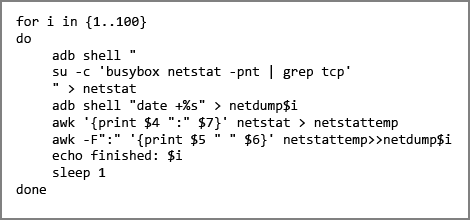
\includegraphics[width=0.75\textwidth]{fig-code-boxed.png}
    \caption{Shell script used for netstat logging.}
    \label{fig:netanalysisshellscript}
\end{figure}


This script calls netstat 100 times, with 1 second interval in between. It filters just the necessary information (port numbers and corresponding pid/package names) from each netstat output, and saves them in separate files, along with the timestamp when the dump was taken. So after executing this script, we had 100 files (namely \texttt{netdump1, netdump2, ... netdump100}). A single netdump file is shown in Fig.~\ref{fig:netdump}.\\

\begin{figure}[h!]
    \centering
    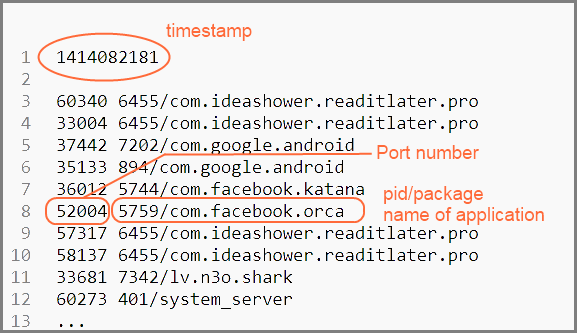
\includegraphics[width=0.75\textwidth]{fig-netdump-a.png}
    \caption{A single netdump file}
    \label{fig:netdump}
\end{figure}

This step requires a rooted android device. Because, being a stripped down variant of linux, Android does not come with the \emph{netstat} executable by default. So we used \emph{Busybox}, a tool that allows execution of all standard UNIX commands in android. Busybox cannot be installed without super user permissions.\\

\subsubsection{Extracting necessary information from packet dump}
Packet dump (.pcap) contains comprehensive meta information about all packets, along with their contents. However, we are only interested in HTTP packets and only three fields of each packet. Pcap filtering can be accomplished by many different ways among which we used Wireshark.\\

We opened the pcap file in Wireshark. Then the following display filter was applied on the dump:
\begin{verbatim}
	http && ip.src == X.X.X.X
\end{verbatim}

Here, \texttt{X.X.X.X} is the IP address of the device. This was used to filter out the http responses. For now, we are only interested in requests.\\
We kept only the following columns in Wireshark:
\begin{itemize}
\item Time (in Seconds since epoch format)
\item Src Port
\item Full Request URI
\end{itemize}
Then we exported the displayed packets summary in a plain text file. In our experiment, we named the file \texttt{filtered.txt} (shown in Fig.~\ref{fig:filtered}).\\


\begin{figure}[h!]
    \centering
    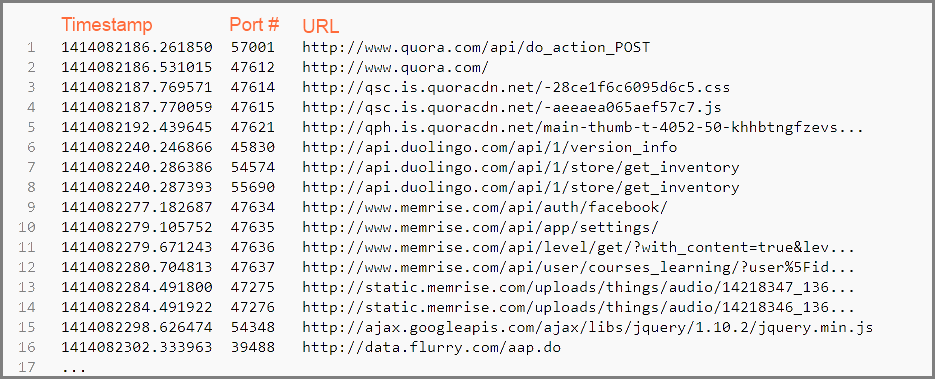
\includegraphics[width=1\textwidth]{fig-filtered-a.png}
    \caption{Extracted information from the packet dump in \texttt{filtered.txt} file}
    \label{fig:filtered}
\end{figure}

% \begin{figure*}[htb]
%     \centering
%     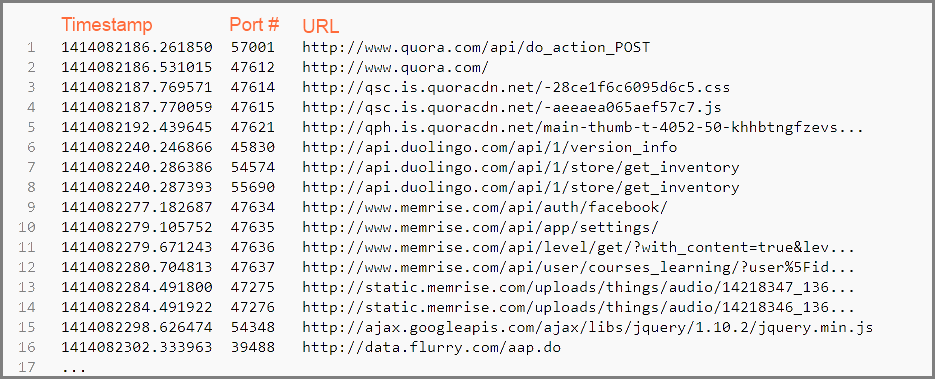
\includegraphics[width=6.0 in]{fig-filtered-a.png}
%     \caption{\texttt{filtered.txt}: Extracted information from the packet dump}
%     \label{fig:filtered}
% \end{figure*}


\subsubsection {Aggregating packet dump and netstat logs}
Before this step, we had 100 files containing netstat outputs (\emph{port-application} mapping at specific times). And we had a file filtered.txt, which contains the \emph{port-URL} mapping for all HTTP request packets. We have written a script which processes all these files to produce the final App-URL table.\\ 

Since netdump files contains \emph{port-app} mappings for specific moments (1 second apart), a packet's time will not necessarily match exactly with any of these moments. To assign such a packet to an application, we have made some assumptions.\\

Let $t$ be the timestamp of a packet. Let $t_1$, $t_2$, $t_3, ... , t_{100}$ are the timestamps of the netstat outputs (they are stored in corresponding netdump files). Of course $t_1 < t_1 < t_3 < ... < t_{100}$ . If $t < t_1$ or $t > t_{100}$, we discard the packet. We only consider packets with $t$ such that $t_1 \leq t \leq t_{100}$.\\

Now for each of these packets, there is an $i$ such that $t_i \leq t$ and $t_{i+1} > t$. We assign a packet to an application using the following rules:
\begin{enumerate}
\item If the same application A was using the packet's port at both $t_i$ and $t_{i+1}$, then application A is the sender of the packet.
\item If application A was using the port at $t_i$, and the port was not in use at $t_{i+1}$, application A originated the packet.
\item If the port was not in use at $t_i$, and application A was holding it at $t_{i+1}$, application A originated the packet.
\item If the port was being used by application A at $t_i$ and application B at $t_{i+1}$ then,\\
	 if $t - t_i \leq t_{i+1} - t$, application A originated the packet. Otherwise application B originated it.
\item If no application was using the port at either $t_i$ or $t_{i+1}$, We discard the packet.
\end{enumerate}
Case 5 indicates that after $t_i$, some application opened the port, sent some packet(s) and then released the port before $t_{i+1}$. So this packet has gone untraced. We can lessen the frequency of such occurrences by decreasing the interval between $t_i$ and $t_{i+1}$.\\

So for every packet (except the ones of case 5), we know the app which originated it. And \texttt{filtered.txt} contains Full request URI of all packets. So we now know the URL specified in the packet was contacted by this application. We have logged these (Application, URL) entries for each packet and the App-URL table is ready. A sample table is shown in Fig.~\ref{fig:final_out}.

\begin{figure}[h!]
    \centering
    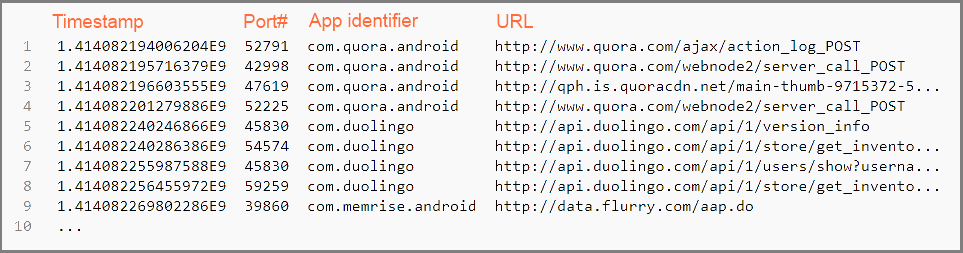
\includegraphics[width=1\textwidth]{fig-output-a.png}
    \caption{Final output: App vs. URL table}
    \label{fig:final_out}
\end{figure}


\subsection{Matching the URLs with Domain-blacklists}
When the App-URL table is ready, the table can be sent to a central server. The server can search the table for already known malicious domains, and notify the android device of any rogue application which might be trying to connect to a blacklisted domain. The server can also enhance its blacklist by adding new domains that are contacted by a malicious application.\\

\section{Results}
We analyzed two known malwares using this method: \emph{DroidKungFu} and \emph{AnserverBot}, both known for contacting remote C\&C servers \cite{zhou2012dissecting}. Within minutes of installation DroidKungFu accessed \emph{www.waps.cn}, which was listed as a malicious domain in \emph{virustotal.com}. Anserverbot did not contact any blacklisted domain within the first 10 minutes when we recorded packets. The reason might be using an unreliable and freely available domain-blacklist from the internet. Or worse, maybe it communicates over protocol(s) other than HTTP.
